\Problem{Skyline}{skyline}
% author: Jimmy M�rdell

\begin{wrapfigure}{r}{5cm}
\vspace{-5mm}

\includegraphics[width=\linewidth,keepaspectratio=true]{skyline/skyline}
\vspace{-9mm}
\end{wrapfigure}

\noindent
Last time I visited Shanghai I admired its beautiful skyline. It also got me thinking, "Hmm, how much of the buildings do I actually see?" since the buildings wholly or partially cover each other when viewed from a distance.

In this problem, we assume that all buildings have a trapezoid shape when viewed from a distance. That is, vertical walls but a roof that may slope. Given the coordinates of the buildings, calculate how large part of each building that is visible to you (i.e. not covered by other buildings).

\Input
The first line contains an integer, $N$ ($2 \le N \le 100$), the number of buildings in the city.\\
Then follows $N$ lines each describing a building. Each such line contains 4 integers, $x_1$, $y_1$, $x_2$, and $y_2$ ($0 \le x_1 < x_2 \le 10 000, 0 < y_1, y_2 \le 10 000$). The buildings are given in distance order, the first building being the one closest to you, and so on.

\Output
For each building, output a line containing a floating point number between 0 and 1, the relative visible part of the building. The absolute error for each building must be $< 10^{-6}$.

\Xample{skyline/skyline.1}

\Xample{skyline/skyline.2}

\begin{figure}
\centering
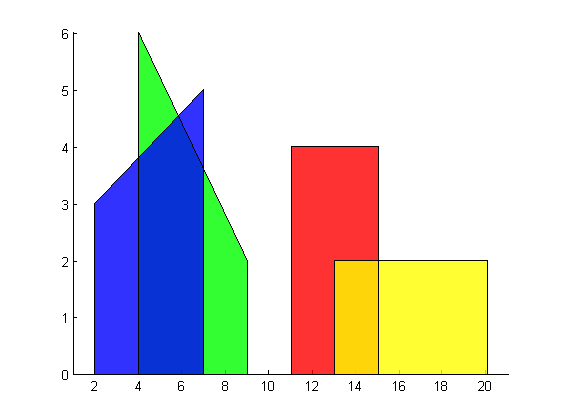
\includegraphics[width=\linewidth,height=150pt,keepaspectratio=true]{skyline/skyline1}
\caption{Figure of the first sample case}
\end{figure}
